\documentclass[12pt]{book}
\usepackage[utf8]{inputenc}
\usepackage[T1]{fontenc}
\usepackage{lmodern}
\usepackage[slovak]{babel}
\usepackage{graphicx}
\usepackage{anysize}
\usepackage{hyperref}
\usepackage{appendix}

\ifpdf
\pdfcompresslevel=9
\else
\usepackage{graphicx}
\fi

\def\mftitle{Domáce účtovníctvo}
\def\mfthesistype{Bakalárska práca}
\def\mfauthor{Peter Kotulič}
\def\mfadvisor{Mgr. Ján Kľuka, PhD.}
\def\mfplacedate{Bratislava, 2013}

\hypersetup{
    bookmarks=true,         % show bookmarks bar?
    unicode=true,          % non-Latin characters in Acrobat’s bookmarks
    pdftoolbar=true,        % show Acrobat’s toolbar?
    pdfmenubar=true,        % show Acrobat’s menu?
    pdffitwindow=false,     % window fit to page when opened
    pdfstartview={FitH},    % fits the width of the page to the window
    pdftitle={\mftitle},    % title
    pdfauthor={\mfauthor},     % author
    pdfsubject={Subject},   % subject of the document
    pdfcreator={\mfauthor},   % creator of the document
    pdfkeywords={accounting, finance, framework, MVC, CakePHP}, % list of keywords
    pdfnewwindow=true,      % links in new window
    colorlinks=true,       % false: boxed links; true: colored links
    linkcolor=blue,          % color of internal links
    citecolor=green,        % color of links to bibliography
    filecolor=cyan,      % color of file links
    urlcolor=blue           % color of external links
}


\renewcommand\baselinestretch{1.3} 

\marginsize{3.5cm}{2cm}{2.5cm}{2.5cm}

\ifx\pdfoutput\undefined\relax\else\pdfinfo{ /Title (\mftitle) /Author (\mfauthor) /Creator (PDFLaTeX) } \fi

\begin{document}

\frontmatter

\thispagestyle{empty}

\noindent
\begin{minipage}{1\textwidth}
\begin{center}
\large\bf UNIVERZITA KOMENSKÉHO V BRATISLAVE\\
FAKULTA MATEMATIKY, FYZIKY A INFORMATIKY\\
\end{center}
\end{minipage}

\vfill
\begin{minipage}{0.8\textwidth}
\begin{center}
\LARGE\bf\sc\mftitle
\end{center}
\end{minipage}
\vfill
{\large\bf 2013}\\

{\large\bf \mfauthor}
\eject

\thispagestyle{empty}~\vfill\eject

\thispagestyle{empty}

\noindent
\begin{minipage}{1\textwidth}
\begin{center}
\large\bf UNIVERZITA KOMENSKÉHO V BRATISLAVE\\
FAKULTA MATEMATIKY, FYZIKY A INFORMATIKY
\end{center}
\end{minipage}
\vfill
\begin{minipage}{0.8\textwidth}
\begin{center}
\LARGE\sc\mftitle \\
\smallskip
\large\bf\mfthesistype
\end{center}
\end{minipage}
\vfill

\begin{table}[h]
  \begin{tabular}{ l }
	Študijný program : Aplikovaná informatika\\
	Študijný odbor: 9.2.9 Aplikovaná informatika\\
	Školiteľ: \mfadvisor \\
	\\
	\\	
	{\large\bf\mfplacedate}\\
	\\
	{\large\bf\mfauthor}
  \end{tabular}
\end{table}

\eject

\thispagestyle{empty}~\vfill\eject

\thispagestyle{empty}

\noindent
\begin{minipage}{1\textwidth}
\begin{center}
Univerzita Komenského v Bratislave\\
Fakulta Matematiky, Fyziky a Informatiky
\smallskip
\end{center}
\end{minipage}
\hrule

\begin{center}
\centerline{\Large \bf Zadanie}
\end{center}

{\bf Meno a priezvisko študenta:} \mfauthor \\

{\bf Študijný program:} aplikovaná informatika \\

{\bf Typ záverečnej práce:} bakalárska \\

{\bf Jazyk záverečnej práce:} slovenský \\

{\bf Názov:} \mftitle \\

{\bf Cieľ práce:} Navrhnúť a implementovať webovú aplikáciu umožňujúcu používateľom udržiavanie prehľadu o príjmoch a výdavkoch ich rodinných rozpočtov v minulosti a jednoduché formy plánovania do budúcnosti. Prispôsobiť najčastejšie potrebné funkcie mobilnému použitiu. Využiť framework pre vývoj webových aplikácií, návrhové vzory a rigorózne testovanie. \\

{\bf Školiteľ:} \mfadvisor \\

\bigskip

\hfill\hbox{ V Bratislave 22. októbra 2012} \hfill\hbox{ \begin{tabular}{c} \\ doc. RNDr. Mária Markošová, PhD.\\ gestor št. programu \end{tabular}} \\

\bigskip

\hfill\hbox{ \begin{tabular}{c} \\ Peter Kotulič \\  študent \end{tabular}} \hfill\hbox{ \begin{tabular}{c} \\ Mgr. Ján Kľuka, PhD. \\ vedúci, resp. školiteľ \end{tabular}}

\eject

\thispagestyle{empty}~\vfill\eject

\section*{Abstrakt}
KOTULIČ, Peter: \mftitle. [\mfthesistype] – Univerzita Komenského v Bratislave. Fakulta matematiky, fyziky a informatiky; Katedra aplikovanej informatiky. – Školiteľ: Mgr. Ján Kľuka, PhD.. 

TODO

{\bf Kľúčové slová: účtovníctvo, financie, framework, MVC, CakePHP}

\section*{Abstract}
KOTULIČ, Peter: Home accounting software. [Bachelor thesis] – Comenius University in Bratislava. Faculty of Mathematics, Physics and Informatics; Department of Applied Informatics. – Supervisor: Mgr. Ján Kľuka, PhD.. 

TODO

{\bf Keywords: accounting, finance, framework, MVC, CakePHP}

\eject

\thispagestyle{empty}~\vfill\eject

{~}\vspace{12cm}

\noindent
\begin{minipage}{0.25\textwidth}~\end{minipage}
\begin{minipage}{0.68\textwidth}
Čestne prehlasujem, že som túto bakalársku prácu vypracoval(a) samostatne s použitím citovaných zdrojov.

\bigskip\bigskip

V Bratislave XX. júna \hfill\hbox to 6cm{\dotfill}
\end{minipage}
\vfill\eject

\tableofcontents

\newpage


\mainmatter

\chapter{Úvod}\label{chap:intro}

\section{Motivácia}
Pri tvorbe tejto práce ma najviac ovplyvnila aktuálna situácia v našej spoločnosti, ktorá je čím ďalej, tým viac konzumne zameraná. Nakupujeme oveľa viac ako v minulosti. A nejde len o potrebné veci. A čím viac vecí nakúpime, tým menší prehľad v nich máme. A tak nakupujeme ešte viac. Tento konzumný spôsob života vplýva najviac na našu peňaženku. A rovnako ako máme problém vyznať sa vo veciach ktoré nakupujeme, rovnako vzniká problém vyznať sa aj v našich financiách. A toto by som rád vyriešil. Verím tomu, že čím viac budeme mať svoje financie pod kontrolou, tým lepšie sa nám bude žiť. Čím lepšie budeme vedieť na čo míňame, tým ľahšie sa nám bude dať naplánovať na ktorých veciach môžeme ušetriť. Mať prehľad a začať spravovať svoje domáce účtovníctvo je tým prvým krokom, ktorý musíme urobiť.

Ďalšou významnou motiváciou k tvorbe tejto práce bola pre mňa túžba naučiť sa niečo nové. Niečo, čoho znalosti mi veľmi dobre poslúžia aj pri mojich budúcich projektoch. V tomto prípade ide o použitie \emph{frameworku} (vývojového rámca) na tvorbu webových aplikácii. Bude sa na ňom zakladať celá moja aplikácia na domáce účtovníctvo.   

\section{Ciele práce}
Hlavným cieľom tejto práce je vytvoriť webovú aplikáciu Domáce účtovníctvo na jednoduchú a prehľadnú správu osobných (domácich?) financií. Keďže je už podobných aplikácii dosť veľa, mojím plánom nebude urobiť len ich jednoduchú kópiu. Budem sa snažiť porovnať tieto existujúce aplikácie, vyhodnotiť ich klady a zápory, a z každej si zobrať len to najlepšie, čo implementujem do mojej výslednej aplikácie. Zamerať sa chcem taktiež aj na jednoduché a prehľadné grafické rozhranie aplikácie, v ktorom sa používateľ bude vedieť orientovať po pár kliknutiach myšou. Toto je jedna z vecí, ktorú by už existujúci podobné aplikácie mali prepracovať. Pri ich skúmaní sa mi často stávalo, že som nevedel a musel dlho hľadať ako vykonať určitú akciu. A toto sa pri aplikáciách, ktoré sú určené bežným používateľom nesmie stávať. Podobným jednoduchým a prehľadným štýlom bude spravená aj mobilná verzia aplikácie. V jednoduchosti je krása. A tak myslím, že je zbytočné robiť prekomplikovanú aplikáciu s \uv{milión} funkciami, keď ju používateľ po piatich minútach vypne, lebo sa v nej nevyzná.


\chapter{Východiská}\label{chap:background}
V tejto časti práce sa budem snažiť opísať východiská, ktoré ma inšpirovali a pomohli mi pri tvorbe bakalárskej práce. Okrem opisu základnej teórie potrebnej na realizáciu práce pôjde aj o prehľad funkčných požiadaviek na výslednú aplikáciu.

Taktiež spravím prehľad už implementovaných, podobných riešení na správu domáceho účtovníctva. Budem sa zaoberať tromi hlavnými typmi aplikácií. Pôjde o webové, mobilné a desktopové aplikácie na správu a prehľad financií v domácnosti. Mojou snahou je zhrnúť základné vlastnosti a funkcionalitu týchto aplikácií, z každej si zobrať to najlepšie a implementovať to do mojej práce v čo najväčšej miere.

Ďalšiu časť tejto kapitoly bude tvoriť popis Model–view–controller architektúry(MVC) \cite{UvodMVC}\ , ktorá bude s pomocou frameworku CakePHP použitá aj v mojej práci. V súčasnosti ide o jeden z najobľúbenejších spôsobov tvorby aplikácií. Keďže som už spomenul aj framework v ktorom budem robiť aplikáciu, rád by som časť tejto kapitoly venoval aj jemu.
Nakoniec by som sa rád pozrel a priblížil aj tému návrhových vzorov, ktoré takáto práca bude vyžadovať.\newpage



\section{Použité webové technológie}
\subsection{HTML a CSS}
HTML \cite{HTML}\ je skratka pre HyperText Markup Language. Je to najpoužívanejší značkovací jazyk na zápis hypermediálnych dokumentov, ktorý používame pri tvorbe web stránok. Štruktúru HTML dokumentu určuje definícia typu (Document Type Definition; DTD). Táto definícia určuje množinu značiek, ktoré môžu byť použité v dokumente. 

Aktuálna verzia tohto jazyka je HTML 5 \cite{HTML5}\ . Táto verzia priniesla mnoho výhod. Okrem tagu video, ktorý by sa mal stať novým štandardom na prezeranie videí a filmov na webe ide hlavne o nové štrukturálne elementy.
 
Element \texttt{div} teraz môže byť nahradený presnejšie definovanými elementami ako sú \texttt{header}, nav, section, article, aside a footer. Na jednej strane to pomáha k prehľadnejšiemu kódu a na druhú stranu aj koncovému používateľovi pri jednoduchšom pohybe na stránke. Napríklad môže ísť o rýchle preskočenie navigácie alebo jednoduchší pohyb medzi rôznymi článkami.

Dalšou novinkou sú nové atribúty ktoré môžeme využiť pri formulároch a inputoch. Pre mňa poslednou dôležitou výhodou HTML 5 ktorú by som rád spomenul je použitie Inline SVG(Scalable Vector Graphics) . Ide o vektorovú grafiku ktorú používa aj mnou neskôr spomínaná javascriptová Highcharts knižnica.

CSS \cite{CSS21}\ (Cascading Style Sheets - kaskádové štýly) je štýlovací jazyk, ktorý popisuje ako budú zobrazené stránky, ktoré boli napísané v (X)HTML. CSS umožňujú vizuálne formátovať webové dokumenty. Vytvárame tak štruktúrované dokumenty v ktorých oddeľujeme obsah dokumentu(HTML) od jeho vzhľadu(CSS). Hlavné z výhod použitia CSS su prehľadnejší kód, menšia dátová náročnosť a jednoduchá zmena formátovania určitých elementov na celej stránke bez nutnosti formátovania každého elementu zvlášť. 

\subsection{CakePHP} 
CakePHP \cite{CakePHP}\ je open source webový framework určený na vývoj webových aplikácií v programovacom jazyku PHP verzie 4 a 5. Tento framework vznikol už v roku 2005 ako reakcia na veľmi obľúbený a úspešný framework Ruby on Rails. Framework CakePHP je postavený na softwareovej architektúre Model-view-controller, ktorý bližšie opisujem v kapitole 2.4.


\subsection{Highcharts plugin} 
Tento plugin \cite{HighchartsPlugin}\ pre framework CakePHP využíva niektoré skvelé možnosti knižnice pre tvorbu grafov Highcharts. Hlavnou výhodou tejto knižnice je, že je kompletne napísaná v JavaScripte. Pre jej fungovanie nie sú potrebné žiadne client side pluginy akými sú napríklad Java alebo Flash. Knižnica Highcharts funguje vo všetkých moderných webových prehliadačoch a nerobia jej problém ani tie mobilné. Ako na Androide, tak aj na iOS. Použitý plugin pre CakePHP je stále vo vývoji, a preto zatiaľ neponúka všetky výhody Highcharts. Základná funkcionalita ktorú poskytuje však plne postačuje na využitie v mojej aplikácii.

\section{Existujúce riešenia}
Pred začatím tvorby svojej aplikácie som urobil prehľad podobných existujúcich riešení. Rozdelil som ich do troch kategórií. Webové aplikácie, desktopové aplikácie a mobilné aplikácie.
Na začiatok by som rád uviedol, že všetky ďalej spomínané aplikácie spĺňali určitú základnú funkcionalitu, ktorú od aplikácie na prehľad rozpočtu berieme za samozrejmú.
\begin{itemize}
\item{pridávanie, editovanie a mazanie jednorazových príjmov a výdavkov}
\item{pridávanie, editovanie a mazanie opakovaných príjmov a výdavkov}
\end{itemize}

\subsection{Webové aplikácie}
\subsubsection{Budget Pulse \cite{BudgetPulse}\ }
\begin{itemize}
\item{jednoduchá administrácia a prehľady}
\item{komplikovanejšie/menej prehľadné pridávanie výdavkov a príjmov}
\item{základná funkcia v aplikácii je pridanie transakcie, v následnom menu si používateľ vyberie či ide o príjem alebo výdavok, určí jeho kategóriu, popis, sumu, množstvo, konto(účet) ktoré chce použiť, dátum, prípadné zadanie opakovania transakcie}
\item{možnosť rozdelenia transakcie na menšie časti a ich priradenie do rôznych kategórií}
\item{možnosť pridania viacerých kont}
\item{dáta import, export}
\item{grafy a prehľady:}
\begin{itemize}
\item{koláčový graf (kategórie za určité obdobie)}
\item{stĺpcový graf (kategórie/suma za určité obdobie)}
\item{tabuľkové prehľady (kategórie/čas)}
\end{itemize}
\item{možnosť určenia osobných cieľov (používateľ si nastaví sumu, ktorá sa mu napríklad raz za mesiac odčíta z konta a priradí k určitému osobnému cieľu, na ktorý si chce našetriť)}
\end{itemize}

\subsubsection{Buxfer \cite{Buxfer}\ }
\begin{itemize}
\item{oveľa prehľadnejšia aplikácia ako budgetpulse}
\item{veľmi dobre spracovaná a prehľadná hlavná stránka}
\begin{itemize}
\item{zobrazuje stav účtu, výdavky za posledný mesiac koláčovým grafom}
\item{prehľad mesačného budgetu podľa kategórií}
\item{pripomienky o budúcich výdavkoch (grafický mesačný kalendár)}
\item{tabuľkové zobrazenie transakcií (popis, suma, tagy, účet, dátum)}
\item{prehľad požičaných peňazí}
\end{itemize}
\item{pridávanie transakcií (príjem, výdavok, transfer, refund), upload výpisov z banky}
\item{grafy a prehľady:}
\begin{itemize}
\item{koláčový graf (kategórie za určité obdobie)}
\item{stĺpcový graf (čas(x)/suma(y))}
\item{tabuľkové prehľady (popis, suma, tagy, účet, dátum), možnosť zatriedenia podľa dátumov alebo sumy}
\end{itemize}
\item{vypočítavanie prehľadov do budúcna na základe predchádzajúcich príjmov a výdavkov}
\end{itemize}


\subsection{Desktopové aplikácie}
\subsubsection{RQ Money \cite{RQMoney}\ }
komplexný správca financií od slovenského autora vytvorený v Delphi
\begin{itemize}
\item{podrobná evidencia transakcií (príjmov, výdavkov a presunov)}
\item{filtrovanie, radenie a sumarizácia záznamov podľa vlastného výberu}
\item{plánovanie transakcií s možnosťou prezerania platobného kalendára}
\item{prehľadné tlačové zostavy, exporty tabuliek (napr. pre MS Excel) a grafov}
\item{porovnanie plánovaných a skutočných transakcií za mesiac}
\item{v štatistike podrobné prehľady za rôzne časové obdobia (tabuľky i grafy)}
\item{možnosť použiť vlastné SQL príkazy}
\item{obsahuje viacjazyčnú podporu}
\item{každá transakcia je spojená s účtom, osobou a kategóriou}
\end{itemize}

\subsection{Mobilné aplikácie}
Zaoberal som sa len aplikáciami pre systém Android
\subsubsection{Easy Money - Android \cite{EasyMoney}\ }
\begin{itemize}
\item{rôzne typy účtov (napríklad cash, kreditná karta, účet v banke,...)}
\item{pridávanie transakcií (názov, cena, kategória, dátum, príjem alebo výdavok, nastavenie opakovania, možnosť rozdelenia transakcií do viacerých kategórií, prevod medzi účtami)}
\item{prehľady:}
\begin{itemize}
\item{príjmy alebo výdavky podľa kategórií (stĺpcové grafy)}
\item{mesačný zoznam príjmov a výdavkov (mesiac(x)/suma(y))}
\item{denné porovnanie príjmov a výdavkov}
\end{itemize} 
\item{pripomienkovač platenia faktúr/účtov}
\item{nastavenie mesačného rozpočtu a prehľad jeho využitia počas mesiaca}
\item{import a export do QIF a CSV}
\item{prehľadávanie medzi transakciami pomocou keywords, triedenie vyhľadávania podľa dátumu, sumy alebo názvu}
\end{itemize}

\subsubsection{Money Lover - Android \cite{MoneyLover}\ }
\begin{itemize}
\item{najprehľadnejšia a najintuitívnejšia mobilná aplikácia, ktorú som testoval}
\item{pridávanie transakcií:}
\begin{itemize}
\item{príjem, výdaj, pôžička alebo dlh}
\item{názov, kategória, suma, poznámka, dátum, účet/konto, nastavenie opakovania (nedá sa nastaviť konkrétny dátum, ale len začiatok alebo koniec týždňa, mesiaca...)}
\end{itemize}
\item{možnosť prehľadu transakcií, kategórií alebo podľa príjmu a výdavkov}
\item{rôzne typy účtov(kont)}
\item{správa dlhov}
\item{plánovanie rozpočtu (plánovanie šetrenia, pridanie rozpočtu na určité časové obdobie – upozornenie pri dosiahnutí určitej hranice)}
\item{sprievodca pri nastavení aplikácie}
\item{grafy a prehľady:}
\begin{itemize}
\item{koláčový graf (kategórie za určité obdobie)}
\item{príjmy verzus výdavky za vybrané obdobie (dátum (x) / suma (y)}
\item{tabuľkové prehľady (popis, suma, tagy, účet, dátum), možnosť zatriedenia podľa dátumov alebo sumy}
\item{tabuľkové mesačné výpisy (príjem, výdaj, dlh, pôžička)}
\end{itemize}
\item{ďalšie možnosti:}
\begin{itemize}
\item{prepočet meny}
\item{výpočet vrcholu}
\item{vyhľadanie bankomatu}
\item{vyhľadanie banky}
\item{počítanie úroku}
\end{itemize}
\end{itemize}

\subsubsection{Expense Manager - Android \cite{ExpenseManager}\ }
\begin{itemize}
\item{pridávanie príjmov a výdavkov}
\begin{itemize}
\item{účet, dátum, suma, názov, popis, číslo účtenky (aj v ostatných aplikáciách)}
\item{možnosť nastavenia predvypĺňaných polí}
\item{pridávanie opakujúcich sa príjmov a výdavkov}
\end{itemize}
\item{pridávanie rozpočtu na opakujúce sa dopredu určené obdobie}
\item{grafy a prehľady:}
\begin{itemize}
\item{príjmy alebo výdavky podľa kategórií (koláčový alebo stĺpcový graf)}
\item{príjmy alebo výdavky podľa mesiacov (dátum (x) / suma (y)}
\item{prehľady podkategórií (koláčový alebo stĺpcový graf)}
\item{vytvorenie vlastného grafu podľa zadaných kritérií (dátum od/do, príjem, výdavok, rozdiel, typ grafu)}
\end{itemize}
\item{ďalšie možnosti:}
\begin{itemize}
\item{kalkulačka}
\item{prepočet meny}
\item{výpočet sprepitného}
\item{Výpočet zľavy a dane}
\item{Výpočet splatenia dlhov na kreditnej karte}
\end{itemize}
\end{itemize}

\subsection{Porovnanie s mojimi cieľami}
Mojim hlavným cieľom je vytvoriť prehľadnú a užívateľsky jednoducho ovládajúcu sa aplikáciu. Všetky spomenuté podobné riešenia sa to tiež snažili splniť. Nie každému sa to však podarilo. Väčšina z aplikácií obsahovala okrem základnej funkcionality aj možnosti, ktoré bežný používateľ asi nikdy nevyužije. To by nevadilo, pokiaľ by tým aplikácia nestrácala na prehľadnosti. Bežný používateľ nemá čas a chuť zisťovať a učiť sa nanovo ovládať aplikáciu. Je zvyknutý na určité ovládacie prvky a ich prehľadné rozloženie. Napríklad pri aplikácii Budgetpulse je problém vykonať aj tú najzákladnejšiu akciu akou je pridanie novej transakcie. A keď to užívateľ konečne nájde, zistí, že rovno pod sebou ma 2 odkazy na pridanie transakcie pričom oba vykonajú rovnakú akciu. Toto riešenie je ideálne ak sa tvorcovia snažia ešte viac domýliť používateľa. A toto je len jedna z množsta vecí, ktoré sa dajú urobiť oveľa lepšie. V jednoduchosti je krása.

Druhou veľkou zmenou oproti ostatným riešeniam bude vytvorenie mobilnej webovej verzie mojej aplikácie. Existujúce riešenia boli zamerané vždy na určitý segment. Išlo vždy buď o webovú, desktopovú alebo mobilnú aplikáciu. Mobilná aplikácia nebola prepojená s webovým riešením a opačne. Tým, že vytvorím aj mobilnú webovú verziu odvodenú od klasickej webovej aplikácie bude tento problém vyriešený. Poslednou veľkou zmenou bude možnosť importu bankových výpisov, čím používateľovi uľahčím zadávanie nových transakcií do aplikácie. Túto možnosť u nás neposkytovala žiadna zo skúšaných aplikácií.

\section{Model–View–Controller}
Pri tvorbe aplikácie budem využívať pravidlá softvérovej architektúry Model–view–controller (MVC) \cite{MVCdevbook}\ . Ide o spôsob architektúry pri ktorom je oddelený dátový model aplikácie(model), používateľské rozhranie aplikácie(view) a riadiaca logika(controller) do 3 komponentov. Táto architektúra zabezpečuje, že úprava niektorého komponentu má len minimálny vplyv na ostatné komponenty. Tým dosahujeme možnosť nezávislého vývoja, testovania a upravovania každého komponentu samostatne.

Hoci MVC architektúra neeliminuje všetky problémy, poskytuje nám základný pevný bod od ktorého sa môžeme odraziť.

\subsection{Model}
Model je dátovým a funkčným základom celej aplikácie. Pozostáva z aplikačných dát a biznis logiky. Komunikuje s databázou a spracováva dáta. Model vôbec nevie o výstupe a tak nemá s konkrétnou prezentáciou nič spoločné. Funguje tak, že prijme parametre z vonku, spracuje ich a potom pošle dáta von. 

Framework CakePHP používa ORM(Objektovo relačné mapovanie) pri ktorom korešpondujú modely s databázovými tabuľkami. Máme teda napríklad model \texttt{Clanok} alebo \texttt{Komentar}. Inštancie modelov obsahujú atribúty z databázy. Článok má napríklad atribút názov. Triede taktiež môžeme definovať metódy inštancií.

Asi najväčšia výhoda v použití modelu je jednoduchá úprava tabuliek v databáze.  Ak by sme ručne písali SQL dopyty, tak by sme v každom z nich museli upraviť zoznam stĺpcov tak, ako sme ich upravili v databáze. Model nám v tomto zásadne pomôže. Postačí nám spraviť úpravu len v ňom.

\subsection{View}
View zabezpečuje zobrazenie výstupu pre používateľa. View získava svoje dáta na zobrazenie priamo z modelu. Model však na komponente View nie je závislý. Používa sa tu však návrhový vzor Observer(Pozorovateľ), ktorý napomáha komponentu Model  informovať ostatné komponenty o zmenách dát. V takomto prípade sa komponent View prihlási komponentu Model ako príjemca týchto informácií. V jednoduchosti sa to dá zhrnúť tak, že Observer sa používa pre View, keď je potrebné sledovať Model.



\subsection{Controller}
Controller(radič) je časť MVC architektúry ktorá reaguje na udalosti, ktoré väčšinou pochádzajú od užívateľa a postará sa o zmeny v modely a View.  Stará sa o tok udalostí v aplikácii a aplikačnú logiku. Controller teda prijíma všetky zmeny od užívateľa a postará sa o ich vykonanie. Ak vykonaná akcia požaduje zmenu údajov, požiada o to model. Ten podľa vstupných parametrov prevedie požadovanú akciu a upozorní na to View. View zobrazí upravené dáta pre užívateľa.

Pri niektorých typoch implementácie MVC môže Controller priamo komunikovať s View. Controller môže v tomto prípade rozhodovať ktoré View sa majú zobraziť. Jeho hlavnou schopnosťou však naďalej ostáva schopnosť Controlleru upraviť model.

Pri webovej implementácii MVC frameworku sa Controller najčastejšie skladá z dvoch hlavných častí. Prvou časťou je front controller. Tento Controller zachytí všetky http požiadavky, spracuje ich a potom pošle konkrétnym Controllerom. Druhá hlavná časť sú tieto konkrétne Controllery. Controller prijme dáta, ktoré pôvodne pochádzali z http pôžiadavky, uloží ich do Modelu a ten nasmeruje na špecifický View. Ten tieto spracované dáta zobrazí pre používateľa.

\subsection{MVC verzus Passive View MVC}
Ako som už spomínal vo východiskách, moja práca bude založená na frameworku CakePHP. V predchádzajúcej časti som opisoval časti z ktorých je zložená MVC architektúra. CakePHP a podobné webové frameworky však nepoužívajú klasickú MVC architektúru. Sú založené na od nej odvodenej architektúre s názvom PMVC (Passive Model View Controller). Základný rozdiel je v tom, že View v tomto modeli len pasívne zobrazuje dáta. View môže byť šablóna napísaná v niektorom zo šablónovacích jazykov. Samotné PHP, ktoré používa CakePHP je tiež šablónovací jazyk. Často sa však používajú aj iné: 


\begin{description}
\item [Smarty] \cite{Smarty}\  je jeden z najznámejších šablónovacích jazykov. Je to samostatná šablónovacia knižnica. Smarty nenahrádza PHP, ale len ho dopĺňa. Jeden z jeho hlavných kladov je jednoduchá syntax.
\item [Savant] \cite{Savant}\  je ďalším známym šablónovacím jazykom. Ako šablónovací jazyk je v ňom použité PHP. Tento jazyk nekompiluje, pretože skripty šablón sú napísané v PHP.
\item [Latte] \cite{Latte}\  je u nás veľmi známy šablónovací jazyk, ktorý používa český framework Nette. Dovoľuje nám vytvárať a používať vlastné makrá. Je rýchlejší ako Smarty a obsahuje viac možností. Taktiež kladie vysoký dôraz na bezpečnosť. Latte automaticky \emph{escapuje} vypisované premenné.
\end{description}

Spoločnými znakmi týchto šablónovacích jazykov je ich jednoduchá syntax a preklad do jazyka PHP. Ak by sa šablóny prekladali vždy až pri zobrazení aplikácie, boli by zbytočne príliš náročné na výpočet.
\newline

View je najčastejšie phtml šablóna, ktorá obsahuje stránku a tagy určitého značkovacieho jazyka. Vďaka tomu sa už nemusí aktualizovať podľa stavu modelu a ani na neho už nie je priamo napojený. Taktiež nám to dovoľuje zamerať testovanie na Controller bez toho aby sme mali problémy s View. Z tohto vyplýva, že jedným z hlavných kladov tejto architektúry je zlepšenie a zjednodušenie testovateľnosti. \cite{PMVC}\  Kvôli tomuto modelu však vzniká Controlleru ďalšia povinnosť. Musí synchronizovať View a Model. 
\newline

Implementácia PMVC v CakePHP prebieha nasledovne:

\begin{enumerate}
\item na HTTP server je používateľom zaslaná požiadavka cez GET alebo POST dáta a s nimi spojenú URL adresu
\item server túto požiadavku prepošle ďalej dispečerovi, ktorý je implementovaný na vzore Front Controlleru
\item Front Controller ju následne spracuje a zaistí akciu na konkrétnom Controlleri
\item Controller tieto dáta spracuje podľa aplikačnej logiky a vykoná zmeny na Modeli
\item tieto zmeny sa uložia v databáze 
\item Controller si vypýta od Modelu aktualizované dáta a zašle ich na View
\item používateľovi sa zobrazí odpoveď.
\end{enumerate}
 

\section{Návrhové vzory}
V živote sa často stretávame s úlohami a problémami, ktoré musíme vyriešiť. Väčšinou nie sme prví, kto natrafil na konkrétny problém. Našlo sa už veľa ľudí pred nami, ktorí ho vyriešili. A nie je predsa potrebné vymýšľať koleso znovu a znovu. Platí to aj pri tvorbe aplikácií.  Často natrafíme na rovnaké, prípadne aspoň podobné problémy. Takéto situácie nám pri programovaní pomáhajú riešiť návrhové vzory \cite{NavrhoveVzory}\ . Návrhový vzor je overená šablóna alebo popis riešenia problému.

Zvyčajne nám objektovo orientované návrhové vzory definujú vzťahy medzi objektmi a triedami. Nedefinujú nám implementáciu konkrétnej triedy.  

Pozitív použitia návrhových vzorov je pre nás mnoho. Umožňujú nám napísať kód v ktorom sa aj iný programátor dokáže ľahko orientovať. Sú to už časom zabehnuté funkčné spôsoby a tak je menšia šanca, že spravíme chybu. 

Pre objektívnosť spomeniem aj pár negatív. Niekedy sa pozitívne vlastnosti veľmi ľahko zmenia na negatívne. Podľa definície vyžaduje použitie návrhových vzorov dodržiavanie určitých pravidiel pri písaní kódu. Často by sme na implementáciu niektorých funkcií mohli použiť skratku, ale keďže používame návrhové vzory budeme to musieť urobiť tou dlhšou cestou. Občas sa preto oplatí použiť vlastné riešenie.

\chapter{Analýza a návrh}
\section{Funkčné požiadavky}
\subsection{Webová verzia aplikácie}
Funkčnosť webovej aplikácie sa líši z pohľadu rôznych typov používateľov:
\begin{itemize}
\item{Administrátor}
\item{Prihlásený používateľ}
\item{Neprihlásený používateľ}
\end{itemize}

\subsubsection{Administrátor}
Administrátor môže:
\begin{itemize}
\item{Mazať používateľov}
\item{Resetovať heslá po žiadosti používateľa}
\end{itemize}

\subsubsection{Prihlásený používateľ}
Prihlásený používateľ má možnosť kompletnej správy svojich príjmov a výdavkov.
Prihlásený používateľ môže:
\begin{itemize}
\item{Pridávať, editovať a mazať jednorazové príjmy a výdavky}
\item{Pridávať, editovať a mazať opakované príjmy a výdavky}
\item{Možnosť zmeniť jednorazový príjem alebo výdavok na opakovaný a opačne}
\item{Triediť príjmy a výdavky podľa rôznych kategórií, času, podľa toho či sú opakované alebo jednorazové}
\item{prezerať prehľad vývoja stavu financií v čase pomocou grafov}
\item{prezerať  predpokladaný vývoj príjmov a výdavkov na nasledujúci mesiac/rok na základe priemerovania za predchádzajúce obdobie}
\item{prezerať odhady či je vzhľadom na predpokladané príjmy a výdavky možné v budúcnosti splatiť plánované a predpokladané výdavky}
\item{vidieť informácie o tom koľko potrebuje ušetriť na výdavkoch, prípadne navýšiť príjmy pre úspešné zvládnutie platenia budúcich výdavkov}
\item{importovať bankou zaslané výpisy transakcií, ktoré následne aplikácia spracuje a priradí základné kategórie k známym transakciám}
\item{editovať a mazať príjmy a výdavky importované z výpisov transakcií banky}
\item{editovať svoje heslo a e-mail v nastaveniach svojho účtu}
\end{itemize}

\subsubsection{Neprihlásený používateľ}
Neprihlásený používateľ môže:
\begin{itemize}
\item{registrovať sa alebo sa prihlásiť pokiaľ je už registrovaný}
\item{požiadať admina o zresetovanie svojho hesla v prípade jeho zabudnutia}
\end{itemize}
\subsection{Mobilná webová verzia aplikácie}
Funkčnosť mobilnej verzie aplikácie sa líši z pohľadu 2 typov používateľov.
\begin{itemize}
\item{Prihlásený používateľ}
\item{Neprihlásený používateľ}
\end{itemize}

\subsubsection{Prihlásený používateľ}
Prihlásený používateľ môže:
\begin{itemize}
\item{Pridávať, editovať a mazať jednorazové príjmy a výdavky}
\item{Pridávať, editovať a mazať opakované príjmy a výdavky}
\item{Prezerať prehľad vývoja stavu financií}
\item{Triediť príjmy a výdavky podľa rôznych kategórií, času, podľa toho či sú opakované alebo jednorazové}
\end{itemize}

\subsubsection{Neprihlásený používateľ}
Neprihlásený používateľ môže:
\begin{itemize}
\item{registrovať sa alebo sa prihlásiť pokiaľ je už registrovaný}
\item{požiadať admina o zresetovanie svojho hesla v prípade jeho zabudnutia}
\end{itemize}

\section{Používateľské rozhranie}
Ako som spomenul už v časti Porovnanie s mojimi cieľami, v aplikácii Domáce účtovníctvo sa snažím implementovať príjemné, intuitívne a hlavne jednoduché používateľské rozhranie. Na vrch stránky som umiestnil navigáciu so všetkými potrebnými základnými položkami. Pod navigáciou sa v ľavej časti stránky nachadza dodatočné menu s odkazmi na konkrétnejšie podstránky. Okrem nich sa tam nachádzajú aj akcie ktoré možno aplikovať na aktuálnej stránke. Napríklad pri prehľade konkrétnej transakcie sú tam zobrazené možnosti na jej editáciu alebo prípadne na jej zmazanie. Ako som spomenul táto ponuka sa mení v závislosti od vybranej stránky. Pri prehľadoch transakcií sa v tejto časti nachádza nastavenie filtra, podľa ktorého sa zobrazia transakcie.

Napravo od tohoto menu sa nachádza obsah stránky. Pri prehľadoch ide zvyčajne o graf pod ktorým je umiestnená tabuľka s možnosťou triedenia podľa stípcov a jednoduchého stránkovania.


\section{Databázový model}
\subsection{Transactions}
Pre aplikáciu Domáce účtovníctvo sú najdôležitejšou časťou transakcie. Rovnako je pre databázový model najvýznamnejšia tabuľka \texttt{transactions}. Táto tabuľka uchováva informácie o všetkých transakciách. Transakcie sú rozdelené na príjmy a výdavky podľa \texttt{transaction\_type\_id} a preto na to nie je nutné 2 špeciálne tabuľky. \texttt{Transactions} obsahuje cudzie kľúče na stľpce v tabuľkách \texttt{transaction\_types}(\texttt{transaction\_type\_id}), \texttt{categories}(\texttt{category\_id}), \texttt{subcategories}(\texttt{subcategory\_id}), \texttt{users}(\texttt{user\_id}) a dokonca aj sama na seba. To využíva pri opakovaných transakciách odkazovaním na svoj stĺpec \texttt{original\_transaction\_id}.
\subsection{Users}
Druhou významnou tabuľkou(modelom??) sú users(používatelia?), ktorí sú reprezentovaní v tabuľke \texttt{users}. Nájdeme v nej všetky informácie týkajuce sa použivateľa. Zaujímavá je položka active. Určuje či je používateľ stále aktívny a má prístup do systému. V prípade zrušenia konta sa zmení len táto položka a tým je používateľovi zablokovaný ďalší prístup do aplikácie. Táto tabuľka obsahuje jediný cudzí kľuč \texttt{user\_type\_id}, ktorý sa vzťahuje na stĺpec \texttt{id} v tabuľke \texttt{user\_types}. Ďalej je v tejto tabuľke zadefinovaný vzťah hasMany na tabuľky \texttt{transactions}, \texttt{categories}, \texttt{subcategories} a \texttt{imports}. Z toho vyplýva, že jednému používateľovi môže prislúchať viacero záznamov z týchto tabuliek.
\subsection{Categories}
Jednoduchá tabuľka obsahujúca informácie o kategóriách transakcií. Obsahuje len jeden cudzí kľúč \texttt{user\_id} na na stĺpec \texttt{id} v tabuľke \texttt{users}. 
\subsection{Subcategories}
Tabuľka obsahujúca informácie o podkategóriách. Na rozdiel od \texttt{Categories} obsahuje okrem cudzieho kľúča aj ďalší cudzí kľúč \texttt{category\_id} odkazujúci na kategóriu ktorej patrí. 
\subsection{User\_types}
Tabuľka \texttt{user} types slúži na identifikáciu a pomenovanie typu používateľa. Aktuálne sú možné 2 typy používateľov. Admin a bežný používateľ.
\subsection{Transaction\_types} 
Tabuľka \texttt{transaction\_types} slúži na identifikáciu a pomenovanie typu transakcie. Tie sú rozdelené na príjmy a výdavky.
\subsection{Imports} 
Tabuľka obsahujúca len jeden cudzí kľúč \texttt{user\_id}, ktorý definuje vzťah \texttt{belongsTo} k tabuľke \texttt{user} a konkrétnemu userovi(používateľovi).
\begin{figure}[ht]
  \centering
      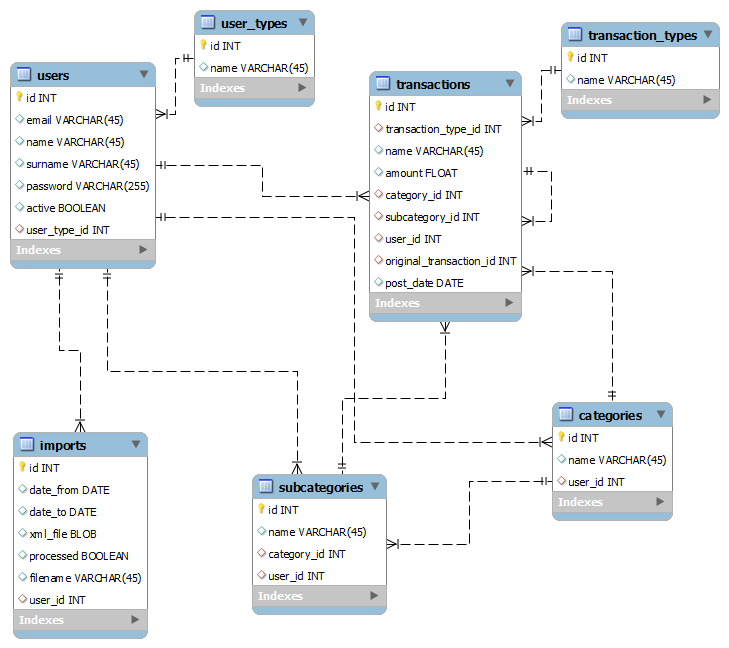
\includegraphics[width=15cm]{databazovy_model}
  \caption{Domáce účtovníctvo - Databázový model}
  \label{DataModel}
\end{figure}  


\chapter{Implementácia}
TODO

Vystupy pre highcharts plugin - rozne typy prehladov podla casovych obdobi (den, mesiac, rok)


\chapter{Záver}\label{chap:outro}
 
Zaverecny popis.

\backmatter

\nocite{*}
\bibliographystyle{abbrv}
\bibliography{literatura}


\newcommand{\dbappendix}[1]{\chapter{#1}}
\appendix
\dbappendix{Príloha}\label{appA}
{\large Priložené DVD médium}\\

Priložené DVD obsahuje:\\
\begin{itemize}
\item Text tejto práce vo formáte TEX a PDF
\item Zdrojové súbory aplikácie Domáce účtovníctvo:
	\begin{itemize}
		\item {\em nieco} - nieco
	\end{itemize}
\end{itemize}

\end{document}
